\chapter{Stopnie i sprawności}
\section{Stopnie harcerskie}
\begin{wrapfigure}{l}{4cm}
  \begin{center}
    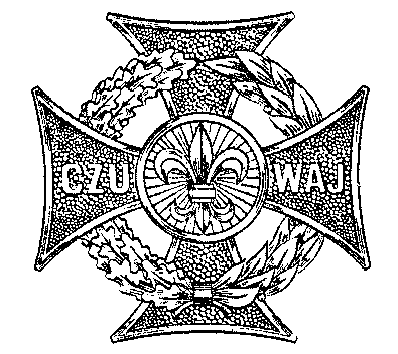
\includegraphics[width=4cm]{grafiki/krzyz.png}
  \end{center}
\end{wrapfigure} 
Każdy z nas zdobywa stopnie. Od chwili gdy przychodzimy na pierwszą zbiórkę, zaczynamy mozolnie wspinać się po drabinie harcerskiego życia, zdobywając szczebel po szczeblu kolejne stopnie. Pokazują one nie tylko ile drogi za nami,  ale przede wszystkim są drogowskazami w marszu do szczytu  ideałów.
	Nasz stopień staje się tak prawie ważny jak imię i nazwisko (wszak wymawiane jednym tchem), starajmy się abyśmy mogli być  z  niego dumni! Kiedy dostanę Krzyż, czy stopień? To pytanie stawiane często starszym druhom przez nowych chłopców w drużynie.  Pamiętajmy Krzyża Harcerskiego, stopnia się nie dostaje, trzeba go zdobyć i bynajmniej nie gadaniem o nim, tylko dobrze przygotowaną i zrealizowaną próbą. Zdobywanie nowego stopnia możemy podzielić na kilka etapów.  Oto one :


1.
Harcerz  przychodzi  do  drużynowego  albo Kapituły stopni (jeśli taka działa w drużynie) i zgłasza swoją  chęć  zdobywania  stopnia. Oczywiście  ktoś może mu to podpowiedzieć,  ale to musi być jego decyzja

2.
Chłopiec  przez  okres  kilku  miesięcy  pracuje  nad  sobą,  w   myśl  wskazówek drużynowego  lub  opiekuna  stopnia, stara  się  dostosować do wymagań stopnia.

3.
Drużynowy  opiekun lub Kapituła stopni  po  ocenie poprzedniego  etapu, uzgadnia  z harcerzem próbę  składającą się  z  ok. 10  zadań obejmujących  różne  dziedziny. Próba  jest  bardzo indywidualna (tak  jak  nie  ma  dwóch Jarków  Wiśniewskich, tak  nie ma dwóch takich samych prób), jak  też  bardzo  konkretna (więc nie ma  zadań  w  stylu powiadomił kogoś  w  ważnej sprawie, ale  np. powiadomiłem  druha Jacka  o  biwaku w  dniu  10 X). Wielką pomocą jest tutaj książeczka z regulaminem stopni harcerskich, która na pewno ma twój drużynowy, a którą może by było warto, abyś posiadał. Tam możesz zaznajomić się z ideą stopnia i wymaganiami na jego zdobycie.

4.
Otwarcie  próby  ogłasza  drużynowy  rozkazem (dla stopni HO - hufcowy, a dla stopnia HR - komendant  Chorągwi), a może  być  zamknięta   z  wynikiem  pozytywnym lub  negatywnym. Próba  trwa  ok. 3 - 12  miesięcy.

5.
Ostatni etap to próba końcowa trwająca 1 do 3 dni. Jest to jakiś wyczyn pokazujący, że ten  harcerz  siłą  charakteru, duchem i zaradnością  udowodnił,  że  jest  wzorowym   np. wywiadowcą.
Zdobyty  stopień   przyznaje  drużynowy, hufcowy (ćwika  i   Harcerza Orlego) lub komendant  Chorągwi (Harcerza  Rzeczypospolitej).


\section{Sprawności harcerskie}


\begin{wrapfigure}{l}{3cm}
  \begin{center}
    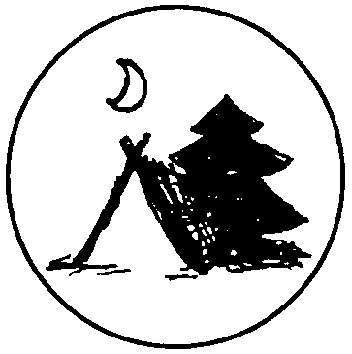
\includegraphics[width=3cm]{grafiki/sprawnosc.png}
  \end{center}
\end{wrapfigure} Zbliżamy się powoli do naszego szczytu Siula Grande. Zdobywanie sprawności, jest niezwykle ważnym elementem harcerskiej kariery. Oczywiście chodzi tu o karierę w  doskonaleniu  samego  siebie. Osobą, mającą nieoceniony wpływ na zdobywanie sprawności w Twojej drużynie masz Ty Druhu Zastępowy. Nie każdy harcerz, od razu wpadnie na pomysł jaką sprawność może zdobyć. Nie każdy drużynowy, znajdzie tyle czasu, aby zajmować się wszystkim w drużynie. Dlatego Roland Philips wymyślił system zastępowy. To ty swoją służbą - Druhu  Zastępowy  pomagasz  zarówno harcerzom z zastępu jak i odciążasz drużynowego.

\noindent
	Zatem w przypadku zdobywania sprawności musisz: 

1. Wiedzieć co to jest sprawność.

2. Wiedzieć jak sprawność należy zdobywać.

3. Umieć przeprowadzić próbę na sprawność.

4. Posiadać własny egzemplarz regulaminu sprawności.

5. Znać go jak najlepiej.

Ad.1
Sprawność - jest to umiejętność, którą harcerz potwierdził  wykonując konkretne dzieło, zadanie. To musi  być  coś  porządnego. Podczas zdobywania sprawności nie ma czasu na naukę. Próba  sprawności jest swojego rodzaju egzaminem.

Ad. 2
Jak  zdobyć sprawność? Najpierw zapytaj samego siebie co chcesz zrobić? Najlepiej gdy Twój pomysł pasuje do realizowanego planu pracy drużyny, obozu, czy warunków  zewnętrznych. Trudno bowiem latem zdobyć sprawność Eskimosa. Po dokonaniu wyboru musisz  przeanalizować wymagania i nie przepisywać ich, tylko ułożyć konkretne zadania. Zadania te musi jeszcze zatwierdzić drużynowy lub Kapituła. Następnie  po  zatwierdzeniu najlepiej jak potrafisz wykonujesz zadania i już zdobyłeś sprawność. Teraz tylko rozkaz drużynowego i maksymalnie 3 dni na wyszycie sprawności na rękawie munduru! To  wszystko dotyczy Ciebie. Jeżeli sprawność zdobywa harcerz z Twojego zastępu, Ty  wiedząc więcej powinieneś mu  pomóc w dojściu do otwarcia próby. Dalej jednak musi sobie radzić sam.

Ad. 3
Jako zastępowy możesz mieć powierzone  przeprowadzenie części, a nawet całej  próby. Pamiętaj, że sprawność zdobywa się konkretnym działaniem, a nie gadaniem. W takiej sytuacji trzeba być bardzo konsekwentnym i wymagającym. Taką postawę trzeba  jednak łączyć  z  życzliwością! Pamiętaj, że sprawności przestają być atrakcyjne zarówno gdy próby  są zbyt trudne  jak  i  wtedy gdy próby  są  zbyt  łatwe.

Ad. 4
Jeżeli jeszcze nie masz Regulaminu sprawności, to natychmiast zażądaj od drużynowego, by ułatwił Ci kupienie go.

Ad. 5
Zanim zaczniesz wymądrzać się na temat zdobywania sprawności, przeczytaj kilka razy regulamin (całość ze wstępem i komentarzem!).

I jeszcze jedno\ldots Pamiętaj, że jako zastępowy powinieneś mieć kilka krążków więcej na rękawie munduru, niż inni harcerze z zastępu. Pomagając innym zdobywać sprawności, nie zapominaj o swoich próbach!

Oto wymagania na dwie sprawności  jednogwiazdkowe. Spróbuj w oparciu o te wymagania ułożyć zadania do próby.
\paragraph{Łącznik:}	\begin{itemize}[noitemsep,nolistsep] 
\item  bezbłędnie  przekazał ustny meldunek lub rozkaz złożony z kilkunastu słów
 \item zaadresował  list z użyciem kodu pocztowego, wypełnił blankiet telegramu, listu  poleconego, przekazu pieniężnego
\item  zapisał wiadomość korzystając z szyfru lub alfabetu Morse’a
\item  pełnił służbę łącznika w trakcie gry terenowej, zwiadu, wycieczki, okolicznościowej uroczystości.
\end{itemize}
\paragraph{Sobieradek obozowy:}	\begin{itemize}[noitemsep,nolistsep] 
\item  zaprojektował i wykonał drobny przedmiot pionierki obozowej (drogowskaz,  ławka,  wieszak, itp.)
\item  przygotował teren pod ognisko, ułożył  je i zamaskował po nim teren
\item  w pracach pionierskich  posłużył  się: piłą, toporkiem, młotkiem, potrafi je zakonserwować po skończonej pracy
\item  wraz z zastępem wykonał wnętrze swojego namiotu
\item  w pracach pionierskich posługiwał się swoimi wymiarami (rozstaw palców długość od końca dłoni do końca łokcia itp.)
\item  rozbił samodzielnie namiot  dwuosobowy, a z zastępem dziesięcioosobowy, w razie czego okopał go.
\item  wykazał umiejętności pionierskie stosując węzły
\end{itemize}